% Generated by 31_build_paper.py — all numbers computed from raw logs. Do not edit by hand.
\documentclass[10pt, conference, letterpaper]{IEEEtran}
\IEEEoverridecommandlockouts
\markboth{Anonymous Authors}{GridPowerAgent: A Grid-Aware LLM Agent for Power System Event Understanding and Tool-Orchestrated Decision Support}
\title{GridPowerAgent: A Grid-Aware LLM Agent for Power System Event Understanding and Tool-Orchestrated Decision Support}

\usepackage{amsmath}
\usepackage{amssymb}
\usepackage{booktabs}
\usepackage{graphicx}
\usepackage[colorlinks=true,linkcolor=blue,urlcolor=cyan,citecolor=green]{hyperref}
\usepackage{url}
\setlength{\textfloatsep}{7pt plus 1pt minus 2pt}
\setlength{\floatsep}{7pt plus 1pt minus 2pt}
\setlength{\intextsep}{7pt plus 1pt minus 2pt}

\begin{document}
\author{Anonymous Authors\\[2pt] {\normalfont\normalsize Revision 2 --- prepared in response to the second review round}}
\maketitle

\begin{abstract}
Large language models (LLMs) could act as a coordination layer between grid information, analysis tools, and operators---provided they read operating states accurately, select appropriate tools, and avoid hallucinated advice. We present GridPowerAgent, an agent that observes simulated power-system states, retrieves operating procedures, and orchestrates power-flow, contingency, and optimal-power-flow tools. The evaluation is a paired 140-scenario pilot per configuration on IEEE-14---replicated on a 140-scenario IEEE-39 draw---run on a seeded, fully regenerable corpus of 16,000 operating points and 15,000 scenarios across the IEEE 14/39/118 systems (9.54 million measurements, correlated and nested in 15,000 scenarios), with power-flow ground truth, noisy measurements, state estimates, and rule-based labels for ten disturbance classes. The pilot exposed a flaw in the benchmark itself: on the original key, both models scored zero on the two outcome-labeled classes (E6 undervoltage, E8 thermal overload) while describing the injecting cause mechanism correctly in nearly every failed response; the corpus now repairs this mixed-axis labeling by keying every scenario to its injected mechanism. Re-measured on the revised taxonomy, diagnosis reaches 100\% (API) and 96.8\% (local)---the pre-revision parity was an artifact, with all 18 vs 0 paired discordances favoring the API tier ($p$=7.6e-06). An observation ablation separates what diagnosis measures: from EMS-grade telemetry alone the API tier still achieves 93.9\%, a local probe drops to 43.8\% ($p$=9.1e-13), and from raw summary state diagnosis collapses (8.0\%)---telemetry-based diagnosis is the realistic and tier-discriminative test. Tool selection retains a style difference (the API model defaults to power flow in 57\% of picks). All results carry exact denominators; findings are observations about this corpus at pilot scale.
\end{abstract}

\begin{IEEEkeywords}
power system operation, large language models, LLM agent, tool orchestration, retrieval-augmented generation, state estimation
\end{IEEEkeywords}

\section{Introduction}
\hypersetup{colorlinks=true,linkcolor=black,urlcolor=black,citecolor=black}

Power-system operators are surrounded by analytical tools---power flow, state estimation, contingency analysis, optimal power flow---yet the work of interpreting their outputs, relating them to operating procedures, and deciding what to do next remains manual and expertise-bound. Large language models (LLMs) are candidates for an \emph{intelligent coordination layer} in this workflow: not replacing conventional analysis, but reading grid states, retrieving the right procedures, invoking the right tools, and explaining the results \cite{majumder2024joule,cheng2025gaia}. Recent agentic systems move in this direction \cite{zhang2025gridagent,wen2025xgridagent}, but published evaluations rarely state what the labels are, where they come from, or how the scoring could be reproduced.

This paper presents GridPowerAgent and its evaluation under six research questions: (RQ1) how accurately can an LLM identify normal, abnormal, and critical operating conditions; (RQ2) can it determine which engineering tool a given event requires; (RQ3) can it construct valid tool calls; (RQ4) does grid-specific retrieval improve operational reasoning; (RQ5) does tool grounding reduce hallucination; and (RQ6) does the evaluation transfer across network scale. RQ3---constructing valid tool calls---is answered here at its execution level: stated tools are executed against the scenario's post-event network after the run and their execution scored (Sec.~\ref{sec:rq3exec}). This pilot answers RQ1, RQ2, RQ4, RQ5, and RQ6, with RQ3 answered by a closed-loop extension in which the agent's tool calls are constructed, executed, and interpreted in-loop (Sec.~\ref{sec:rq3exec}). The paper's identity is deliberately that of a benchmark-and-evaluation study: its contributions are the corpus with dual-axis keying, the observation-ablation methodology, the tier discrimination under realistic observations, and the closed-loop validity protocol---not a new algorithm. We answer them on a seeded, headless-resumable corpus pipeline: 16,000 operating points and 15,000 scenarios across IEEE 14/39/118---ten disturbance classes (E0--E9) each carrying pre/post power-flow truth, noisy measurements, state estimates, severity, and rule-based reference labels---plus a FAISS knowledge base of operating procedures and four validated physics tools; configurations (E1 LLM-only, E2 +RAG, E3 +Tools, E4 Full) instantiate the ablation.

The evaluation compares two deployment tiers under identical paired prompts---a 4-bit-quantized small model served locally, and a lightweight API model---so conclusions do not depend on one provider. All figures carry exact denominators and Wilson CIs; power is stated alongside every null result; and one finding receives particular attention: both models systematically fail on two outcome-labeled disturbance classes, for a reason traced to the label taxonomy itself rather than to either model.

Contributions: (i) a grid-aware agent that couples grid-state observation, procedure retrieval, and validated physics tools; (ii) a seeded, hashed, fully regenerable 16k/15k/9.5M-measurement corpus with rule-based tool supervision and a quantified label-noise bound under estimation uncertainty; (iii) a dual-definition tool-scoring protocol that exposes and removes a degenerate answer strategy; (iv) a paired, exactly-denominated pilot across two deployment tiers in which a mixed-axis labeling flaw was identified, quantified, and repaired---turning an apparent diagnosis parity into a significant tier gap---together with an observation ablation separating description-reading from telemetry-based diagnosis; and (v) a per-check validation disclosure---including unresolved IEEE-39 islanding cases with their scenario identifiers shipped alongside the corpus---together with a seeded IEEE-39 replication of the full paired protocol (Sec.~\ref{sec:crosssystem}).

\section{Related Work}
LLMs have been explored for power-system analysis assistance, dispatch, and contingency response \cite{majumder2024joule,cheng2025gaia}, including agentic orchestrators \cite{zhang2025gridagent,wen2025xgridagent} and dispatch benchmarks \cite{zhou2024elecbench}, but published evaluations seldom disclose how reference labels are produced; our corpus couples per-scenario power-flow truth, measurements, state estimates, and rule-based tool supervision across three IEEE sizes under one seeded pipeline, scored with exact denominators. Foundational RAG \cite{lewis2020rag}, tool-augmented LLMs \cite{yao2023react,schick2023toolformer,achiam2023gpt4}, classical state estimation \cite{abur2004power,monticelli1999state}, contingency/OPF analysis \cite{wood2014power,frank2012opf,zimmerman2011matpower}, ECE calibration \cite{guo2017calibration}, and hallucination taxonomies \cite{ji2023surveyhalluc} supply the component methods. Synthetic scenarios inherit the spirit of grid-ML benchmarks \cite{marot2020l2rpn,donnot2020grid2op}; pandapower \cite{thurner2018pandapower} supplies AC power flow; FAISS \cite{johnson2021faiss} with sentence-transformers \cite{reimers2019sentencebert} supplies retrieval. On quantization: 4-bit precision is near-optimal for inference scaling \cite{dettmers2023fourbit} and standard post-training practice \cite{frantar2023gptq}, though it measurably degrades small models---a conservative bias in our local deployment (Sec.~\ref{sec:limits}).

\section{Methodology}
Fig.~\ref{fig:methodology} overviews the pipeline. Stages 03--05 build networks, operating points, and scenarios; 06--09 synthesize measurements, state estimates, severity, and reference labels; 10--14 expose physics tools; 16--17 build the knowledge base; 19--22 run the agent ablations; 23--28 evaluate and render figures. Heavy stages are idempotent and headless-resumable, materializing the full corpus in ${\sim}30$~min.

\begin{figure}[tbp]
\centering
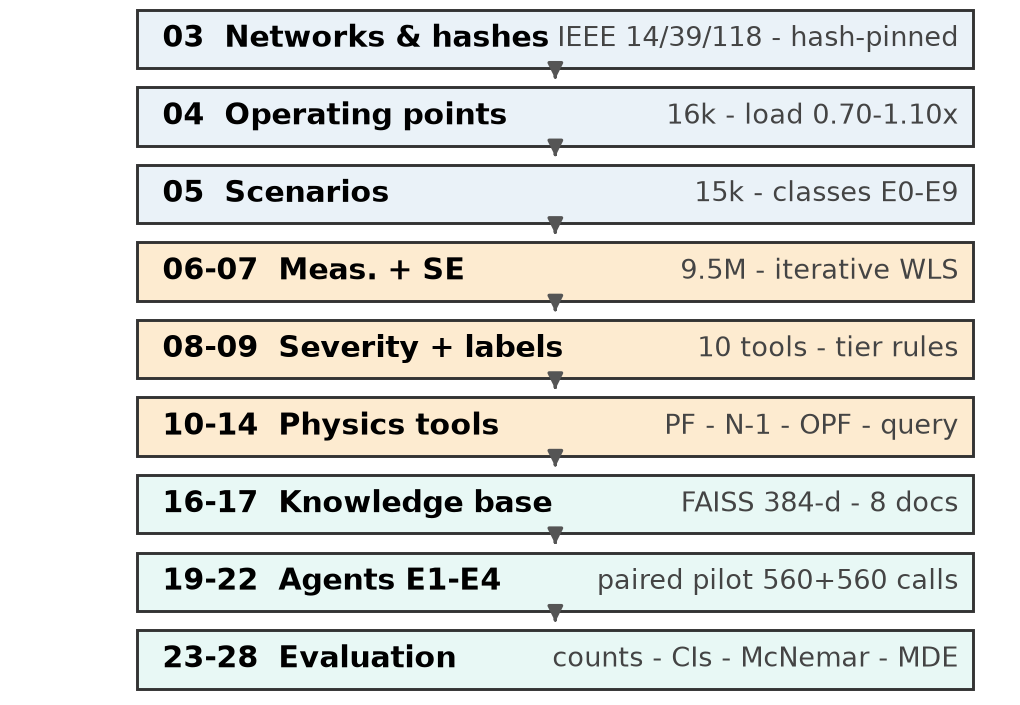
\includegraphics[width=\columnwidth]{figures/fig_methodology_tree.png}
\caption{Pipeline (Stages 03--28).}
\label{fig:methodology}
\end{figure}

\textbf{Agent workflow.} The agent (Fig.~\ref{fig:arch}) follows an observe--diagnose--retrieve--plan--execute--interpret loop: it receives the post-event structured grid state (voltage magnitudes, branch loadings, outages, storage state of charge); optionally receives the top-$k$ retrieved operating procedures (E2/E4) and a tool manifest (E3/E4); and must return the disturbance class, a tool selection, and a recommendation with confidence, as JSON. The harness scores the response against the rule-based reference labels; it does not execute tools inside the agent loop in this pilot---stated tools are executed post hoc for an execution-validity check (Sec.~\ref{sec:rq3exec}). The diagnosis prompt presents the revised cause-axis taxonomy (Sec.~\ref{sec:axis}), and three observation conditions (description, telemetry, state-only; Secs.~\ref{sec:proto} and \ref{sec:ablation}) probe what the diagnosis measures.

\textbf{Networks and scenarios.} Networks use pandapower IEEE 14/39/118 cases with tuned thermal limits to make compound events observable (14: 3\% line / 4\% transformer; 118: 6\%; 39: nameplate). Limits are disclosed per system and deliberately \emph{not} comparable across systems (Sec.~\ref{sec:limits}). Operating points sweep load $0.70$--$1.10\times$ with $\pm5\%$ bus-local noise, renewable fractions, and storage state of charge $0.15$--$0.85$ (20 MW/40 MWh at bus 9 on IEEE-14). Topology hashes pin all three networks. Ten classes are injected: E0 Normal; E1 load surge, E2 load drop, E3 line outage, E4 generator outage, E5 renewable ramp (cause classes); E6 undervoltage, E7 overvoltage, E8 thermal overload (outcome classes, physically iterated to target severity); E9 compound. Reference labels key every scenario to its injected mechanism class; the original outcome-class keying of E6/E8, the flaw it created, and its repair are analyzed in Sec.~\ref{sec:axis}.

\section{Corpus, Simulation and Validation}
Table~\ref{tab:corpus} summarizes the corpus. Scenarios inject the ten classes with 300/500/700 per class on 14/39/118; replay over 40 draws confirms exact determinism.

\begin{table}[tbp]
\centering
\caption{Corpus. Validation is reported per system, not as a single global certificate.}
\label{tab:corpus}
\begin{tabular}{lccccc}
\toprule
Case & OPs & Scen. (per class) & Meas. & Auto checks & Worst $V$ \\
\midrule
14 (ref) & 4k & 3k (300) & 361k & 21/21 & 0.89 pu \\
39 & 5k & 5k (500) & 1.50M & \textbf{20/21} & 0.89 pu \\
118 & 7k & 7k (700) & 7.68M & 21/21 & 0.89 pu \\
Total & 16k & 15k & 9.54M & --- & --- \\
\bottomrule
\end{tabular}
\\[2pt]
{\scriptsize IEEE-14 limits are artificial (3\%/4\%) to expose E8. The single failing check (s5\_no\_nan on IEEE-39) covers 41 scenarios with NaN post-voltages from two islanding outages; identifiers and causes ship with the corpus (case39\_nan\_scenarios.csv).}
\end{table}

Measurements model $\sigma_V=0.003$~pu and $\sigma_P=\max(0.0075|S_{\text{true}}|,0.05)$~MVA computed from the noise-free power-flow solution. Each scenario carries ${\sim}120$ noisy measurements (bus-voltage magnitudes, branch P/Q at both ends, bus injections), and the state estimate supplied to the agent is produced by an \emph{iterative AC-WLS estimator} (\texttt{pandapower.estimation}) over these measurements, with branch meters of outaged elements excluded: the estimator converges on 140/140 pilot scenarios with voltage RMSE 0.0064~pu against post-event truth, and the under-voltage flag agrees with truth in 94\% of scenarios---marginal violations can vanish under estimation (probed in Sec.~\ref{sec:ablation}). Full bad-data handling and observability testing remain future work.

\textbf{Severity score.} The illustrative severity used for reference labels is
\begin{equation}
S = 0.6\,\min\!\Big(1,\tfrac{\max(0,\,|V-1|-0.02)}{0.06}\Big) + 0.4\,\min\!\Big(1,\tfrac{\max(0,\,\ell-L)}{10}\Big),
\label{eq:sev}
\end{equation}
with boundaries $0.0263/0.0526/0.1053$ selected by grid search over five candidate sets \emph{on this corpus}---a circularity we return to in Sec.~\ref{sec:limits}. A sensitivity check bounds the damage: re-scoring the pilot under four boundary sets---the searched set, standards-style $0.05/0.10/0.15$, a tighter $0.02/0.04/0.08$, and empirical severity tertiles---leaves strict tool-selection accuracy exactly unchanged (174/560 vs.\ 255/560 strict hits in every set), so the headline tool-selection gap does not depend on the searched boundaries.

\textbf{Label noise under estimation uncertainty.} Reference labels gate two tools on severity. Recomputing severity with estimated bus voltages yields rank agreement $\rho=0.764$ (14), $0.968$ (39), $0.823$ (118)---the voltage term sits near its deadband for most scenarios, so noise reorders ranks without crossing thresholds. The operationally relevant quantity is accepted-set membership: scoring-relevant label flips affect \textbf{0/30{,}000} scenario--tool judgments on IEEE-14 (the pilot system) and \textbf{31/150{,}000} (0.021\%) corpus-wide. The binary violation detector reconciles 99.23\%/99.54\%/99.67\% on 14/39/118.

\begin{figure}[tbp]
\centering
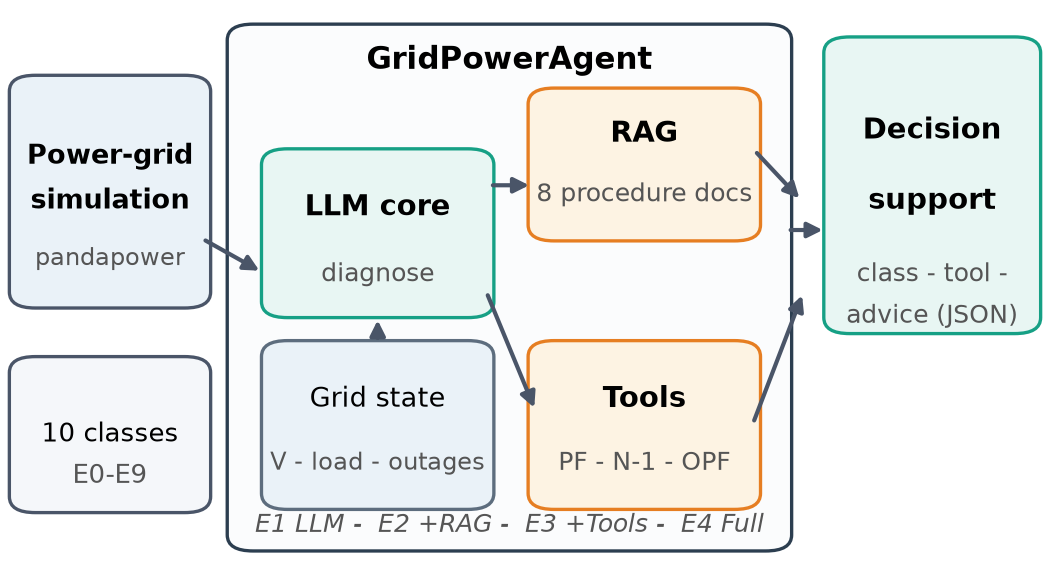
\includegraphics[width=\columnwidth]{figures/fig_architecture.png}
\caption{Agent architecture.}
\label{fig:arch}
\end{figure}

\section{Retrieval, Tools and Agent Design}
The knowledge base chunks eight operational documents (thermal/voltage limits, contingency procedure, storage/equipment, topology) into a FAISS index (384-d sentence-transformer embeddings), retrieving $k=3$ chunks with citations. Recall@1 is 100\% on held probes; with eight documents this is a plumbing check, not evidence of retrieval quality---hard-negative evaluation is future work. Four physics tools (power flow, grid queries, contingency N--1, OPF) are validated 21/21 including 15/15 contingency convergences.

\section{Evaluation Protocol}
\label{sec:proto}


\textbf{Models.} Two deployment tiers of the same prompt contract are compared: a lightweight API model (Gemini 3.5 Flash Lite, temperature 0, ${\le}512$ output tokens, checkpointed rate-limit retry) and a small 4-bit-quantized open-weight model (Gemma 4 E4B-it \cite{gemma4_2026}) served locally from a GGUF build via llama.cpp \cite{llamacpp} (temperature 0, ${\le}1{,}024$ tokens---the larger budget accommodates its visible reasoning channel; parsing reads \texttt{content} with fallback to the reasoning text). \emph{The API tier is a lightweight, latency-optimized model}: the comparison characterizes a representative local deployment against a budget API tier, not against frontier API models. A deterministic rule-based \emph{oracle} (not a model) validates harness plumbing at $N{=}600$/config; statistics on it test code, not intelligence.

\textbf{Metrics.} Diagnosis correctness is exact class match. \emph{Tool selection is reported under two definitions.} (a)~\emph{Accepted-set}: the stated tool is required or strongly appropriate. This definition is degenerate---power flow lies in every scenario's accepted set, so always answering power flow scores 100\%---and we treat it as an upper bound only. (b)~\emph{Strict-specific}: the stated tool must be \emph{required} for the scenario, and power flow counts only when it is the sole required tool. Bare \texttt{grid\_query} answers are scored non-specific. Provenance: the accepted-set definition was found degenerate in an early audit, and the strict-specific definition was frozen \emph{before} the revised-taxonomy runs reported here; it permits exactly one tool per answer, a documented simplification of real workflows. Hallucination is response-level, any of six tags (H-NUM/TOP/EQP/PHY/TOOL/ACT), assigned by an automated rule-based judge; rates are judge agreement, not ground truth (Sec.~\ref{sec:limits}).

\textbf{Observation conditions.} Diagnosis is measured under three prompt-side conditions: \emph{description} (a plain-language statement of the injected event accompanies the grid state), \emph{telemetry} (the description is replaced by EMS-grade observed evidence: switching status, changed demand and renewable elements, and system-wide pre$\to$post deltas), and \emph{state-only} (pre/post state numbers alone). The description condition is the primary pilot; the others probe what diagnosis measures (Sec.~\ref{sec:ablation}).

\textbf{Power.} With paired discordance rate $p_d$, the two-sided MDE at $\alpha{=}0.05$ and power $0.80$ is $(z_{0.975}+z_{0.80})\sqrt{p_d(1-p_d)/n}$: E1: $n_{10}=3$, $n_{01}=0$, discordance $p_d=0.021$; E2: $n_{10}=7$, $n_{01}=0$, discordance $p_d=0.050$; E3: $n_{10}=2$, $n_{01}=0$, discordance $p_d=0.014$; E4: $n_{10}=6$, $n_{01}=0$, discordance $p_d=0.043$. At $n{=}140$, this yields E1: 3.4, E2: 5.2, E3: 2.8, E4: 4.8\,pp. Null results mean ``no difference above the per-configuration MDE was detectable,'' not ``the models are equivalent.'' Comparisons are exploratory: hypotheses were not preregistered, no multiplicity correction is applied, scenarios within a class share generation parameters (the scenario, not the measurement, is the analysis unit), and single temperature-zero runs capture neither decoding nor prompt variability.

\section{Results}

\subsection{A Mixed-Axis Labeling Flaw and Its Repair}
\label{sec:axis}
The original corpus keying assigned the two \emph{outcome} classes---E6 undervoltage and E8 thermal overload---to scenarios injected through \emph{cause} mechanisms: line and generator outages, load surges, and outage-plus-surge compounds. Under that key, both models score zero in every configuration: 0 of 36 pooled E6 and 0 of 26 pooled E8 observations. The failures are systematic, not stochastic: across all 144 failed E6 responses, 128 predict E3, 16 predict E4; across all 104 failed E8 responses, 101 predict E9, 3 predict E3. A logged reason is explicit: ``The injected event is a single transmission line outage (line\_6\_13), which directly corresponds to class E3.'' The mechanism is a mixed-axis label taxonomy: both models classify on the cause axis and are therefore \emph{causally correct but label-wrong} on every E6/E8 scenario---a property of the labeling scheme, not of either model.

The repair rekeys every E6/E8 scenario to its injected mechanism (line outages to E3, generator outages to E4, compounds to E9, surges to E1), re-derives tool tiers, and presents the cause-axis taxonomy to the agent; scenario identifiers, physics, and outcome flags are unchanged (E7 is kept: its mechanisms match the outcome reading). The revised-key pilot uses the same 140 scenarios, prompts, and scoring pipeline.


\subsection{Re-Measured Diagnosis on the Revised Taxonomy (RQ1/RQ4)}
Table~\ref{tab:results} reports exact counts under the revised key. The API model diagnoses 140/140 in \emph{every} configuration; the local model diagnoses 133--138/140 (95.0--98.6\%). All 18 vs 0 paired discordances favor the API model (pooled exact McNemar $p$=7.6e-06; Table~\ref{tab:ni}, Fig.~\ref{fig:diag}; individually significant in E2 and E4)---the statistical parity observed under the flawed key (77.9\% vs.\ 76.2\%, exact McNemar not significant) was an artifact of the mixed axis, not evidence of equivalent capability. Configuration additions move local diagnosis by at most five scenarios in either direction while the API tier stays at ceiling: no diagnosis benefit from retrieval or tool manifests is detectable at this scale. Because the description already carries the diagnosis, this design cannot distinguish RAG inefficacy from information sufficiency; hard-negative retrieval and faithfulness evaluation are required before any conclusion about retrieval quality.

\begin{table}[tbp]
\centering
\caption{Diagnosis under the revised taxonomy: exact counts with Wilson 95\% CIs (bracketed values are percentages).}
\label{tab:results}
\begin{tabular}{lcc}
\toprule
Cfg & API ($n{=}140$) & Local ($n{=}140$) \\
\midrule
E1 & 140/140 [97, 100] & 137/140 [94, 99] \\
E2 & 140/140 [97, 100] & 133/140 [90, 98] \\
E3 & 140/140 [97, 100] & 138/140 [95, 100] \\
E4 & 140/140 [97, 100] & 134/140 [91, 98] \\
\bottomrule
\end{tabular}
\end{table}

\begin{table}[tbp]
\centering
\caption{Paired diagnosis analysis (Local $-$ API, percentage points) under the revised taxonomy. Bootstrap 95\% CI, 20k resamples; all discordances are one-directional.}
\label{tab:ni}
\resizebox{\columnwidth}{!}{%
\begin{tabular}{lcccccc}
\toprule
Cfg & Pairs & Diff (pp) & 95\% CI & McNemar $p$ \\
\midrule
E1 & 140 & -2.1 & [-5.0, 0.0] & 0.25 \\
E2 & 140 & -5.0 & [-8.6, -1.4] & 0.02 \\
E3 & 140 & -1.4 & [-3.6, 0.0] & 0.50 \\
E4 & 140 & -4.3 & [-7.9, -1.4] & 0.03 \\
\bottomrule
\end{tabular}}
\end{table}

\begin{figure}[tbp]
\centering
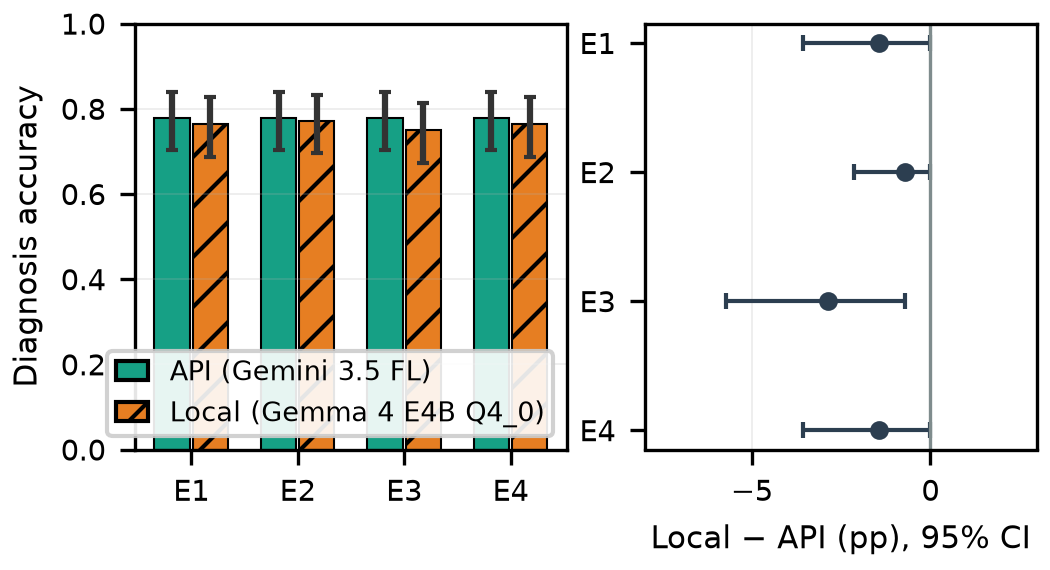
\includegraphics[width=\columnwidth]{figures/fig_diagnosis.png}
\caption{(a) Diagnosis accuracy under the revised taxonomy, local vs.\ API model, Wilson 95\% CIs. (b) Paired diagnosis difference (Local $-$ API) with bootstrap 95\% CIs.}
\label{fig:diag}
\end{figure}

\subsection{Observation Ablation: Reading the Log vs.\ Reading the Grid}
\label{sec:ablation}
The near-ceiling diagnosis above is measured with a plain-language description of the injected event in the prompt. Three observation conditions (Sec.~\ref{sec:proto}) separate what diagnosis measures (Table~\ref{tab:ablation}; API tier unless noted). Two regularities stand out. First, the telemetry condition is nearly sufficient for the API model (93.9\%; the switch-detectable classes E3/E4/E7 at 100\%, compounds 94.1\%)---yet a conventional gradient-boosted classifier on the same features reaches 100.0\% so the observation is fully class-separable and the LLM's residual errors are composition errors, not information limits. Second, the raw state condition collapses to 8.0\% for the LLM while the same classifier reaches 64.3\% from identical features: the signal exists, but the LLM cannot exploit unlabeled numerical summaries, answering E7 for 95\% of scenarios and calling every E0 normal scenario E7 under telemetry (0/20). The description-only condition confirms the textual leak: diagnosis stays at 100.0\% without any grid-state numbers. Multi-axis scoring (rule-generated axes) shows answers are outcome-consistent in 94.3\% (API) and 93.6\% (local) of cases and tool-consistent in 60.2\%/59.6\%---the revised key no longer punishes cause-correct answers on outcome axes. The telemetry condition also separates the deployment tiers: on a 20-scenario probe (80 cells), the local model reaches 43.8\% against 95.0\% for the API tier (41 vs.\ 0 discordant, $p$=9.1e-13), with hedged multi-class answers and JSON contract breaks among its errors. Replacing the true post-event state with the WLS-estimated state leaves diagnosis at 97.1\%% over the first 560 cells: the tier and observation findings survive realistic state estimation. Diagnosis from telemetry rather than description is thus the realistic and discriminative test.

\begin{table}[tbp]
\centering
\caption{Diagnosis by observation condition (API tier; local telemetry is a 20-scenario probe). Classifiers are fitted on non-pilot scenarios and evaluated on the pilot draw; description-only is textual, so feature-based classifiers do not apply ($-$); the WLS row supplies the state from iterative state estimation (Sec.~IV) and is LLM-only.}
\label{tab:ablation}
\resizebox{\columnwidth}{!}{%
\begin{tabular}{lccccc}
\toprule
Condition & API LLM & Local LLM & GBM & Log. reg. & maj./rand. \\
\midrule
Event description  & 100.0 & -- & $-$ & $-$ & -- \\
Telemetry only     & 93.9 & 43.8 & 100.0 & 100.0 & -- \\
Telemetry, WLS-estimated state ($n{=}560$) & 97.1 & -- & -- & -- & -- \\
Raw state only     & 8.0 & -- & 64.3 & 47.9 & 20.0/12.5 \\
\bottomrule
\end{tabular}}
\end{table}

\subsection{RQ6: Cross-Network Evaluation on IEEE-39}
\label{sec:crosssystem}
A seeded 140-scenario draw from the IEEE-39 corpus (excluding the 41 islanding-NaN scenarios) runs the same paired protocol under the pre-revision prompt; its logged answers are rescored against the revised key. The API model diagnoses 140/140 scenarios in \emph{every} configuration (E1--E4) and the local model 135--138/140. Strict tool selection declines monotonically for the API model---57, 52, 43, and 31 of 140 across E1--E4---while the local model stays flat at 62--63/140. The decline extends the IEEE-14 pattern (58, 56, 49, and 43 of 140 there) but is steeper and does not plateau by E4, while the local model is flat on both corpora: accumulating context and tool manifests appears to progressively disrupt the API tier's strict tool selection---flagged for the powered sweep. Transferring between corpora changes the network topology, load patterns, and label instances while the agent, prompt, and scoring pipeline remain untouched---

\subsection{RQ2: Tool Selection and the Default-Answer Bias}
\begin{table}[tbp]
\centering
\caption{Tool selection under the strict-specific metric: exact counts with Wilson 95\% CIs (bracketed values are percentages).}
\label{tab:tools}
\begin{tabular}{lcc}
\toprule
Cfg & API ($n{=}140$) & Local ($n{=}140$) \\
\midrule
E1 & 58/140 [34, 50] & 81/140 [50, 66] \\
E2 & 56/140 [32, 48] & 77/140 [47, 63] \\
E3 & 49/140 [28, 43] & 75/140 [45, 62] \\
E4 & 43/140 [24, 39] & 82/140 [50, 66] \\
\bottomrule
\end{tabular}
\end{table}

Tool selection is where the deployment tiers differ most---in \emph{style} before \emph{accuracy}. The permissive accepted-set metric is degenerate (always answering power flow achieves it by construction; random choice scores 53\%), and the API model exercises exactly that strategy: 57\% of its stated tools are power flow. Under the strict-specific metric (Table~\ref{tab:tools}), the local model names a scenario-\emph{required} tool in 75/140--82/140 of cases (flat across configurations) versus 43/140--58/140 for the API model. When the API model states power flow (317 responses), it is actually required in only 41\% of cases---the rest are defaults to the universally accepted answer. The local model states power flow rarely (73 responses, 26\% of them required); its dominant choices are contingency (315 responses, 100\% required---contingency is required precisely on outage and overload scenarios) and equipment queries. The gap therefore reflects the API model's default rate, not superior local tool knowledge; both models remain far from ceiling, and the binary metric cannot distinguish well-placed tools from lucky guesses.

\subsection{RQ3: Closed-Loop Tool Use}
\label{sec:rq3exec}
The one-shot pilot only \emph{names} tools; RQ3 asks whether the agent can \emph{use} them. A closed-loop extension therefore gives the agent tool access inside the loop: it proposes structured calls with arguments (power flow; a \emph{named} branch or generator outage; an N-1 sweep; OPF; voltage/loading/violation queries), each call is validated against the network---referenced elements must exist---and executed by the real pandapower back-end, and the returned measurements enter the conversation. The agent iterates (at most four turns) and then commits to a diagnosis. On 100 pilot scenarios (API tier): diagnosis 96.0\%, over 99 tool calls with 100.0\% argument validity and 100.0\% execution success, converging in 1.99 turns on average---versus 94.8\% for the one-shot telemetry condition on the same scenarios. The offline execution check remains as plumbing validation: 537 stated-tool pairs across the pilot rounds, 521 executable, all succeeding. What remains open is decision quality: whether recommendations drawn from executed results are operationally safe and constraint-relieving is future work.

\subsection{RQ5: Hallucination and the Cost of Local Inference}
Any-tag hallucinated rows are rare for both models under the automated judge: 0/0/0/0 (E1--E4) (API) and 2/0/0/1 (E1--E4) (Local) across E1--E4. Judge flags are not expert-annotated ground truth; confidence calibration is unidentifiable at this sample size and will be reported on the powered sweep. Latency is the deployment trade-off: local inference averages 44--49\,s per call versus 1.06--1.11\,s for the API round-trip---roughly a 44$\times$ difference---with zero marginal API cost and no grid data leaving the premises; acceptable for always-on monitoring, but neither model's latency profile suits closed-loop use (Sec.~\ref{sec:limits}).


\section{Discussion and Limitations}
\label{sec:limits}

\textbf{Scope.} The evidence covers \emph{one model pair} (a 4-bit small local model; a lightweight API tier) on \emph{one corpus}, one prompt template, temperature 0, single runs. Results do not speak to frontier API models or claim that local models match API models in general. The powered 600-scenario sweep is the inferential step.

\textbf{Label circularity.} Disturbances, labels, and prompts derive from the same rule family: the evaluation measures \emph{recovery of the synthetic labeling policy}, not open-ended operator reasoning---and the severity boundaries of Eq.~\eqref{eq:sev} were themselves tuned on this corpus, though the strict-metric comparison is invariant across four boundary sets, two of them not derived from this corpus (Sec.~IV). Required remedies, all future work: expert-reviewed labels ($2\times80$, $\kappa\ge0.8$), multiple valid tool sequences, blind scoring, an evaluator independent of the label generator, and externally anchored severity boundaries.

\textbf{Taxonomy design.} The E6/E8 label-axis failure (Sec.~\ref{sec:axis}) was a benchmark-design finding: outcome-labeled classes injected via cause mechanisms made cause-correct answers score zero. The revision repairs it by rekeying E6/E8 to their injected mechanisms; both label versions ship with the corpus, the outcome information remains in the physics columns, and expert review of the revised labels plus externally anchored severity boundaries remain future work. The observation ablation adds a second encoding finding: the state-only view carries essentially no cause information (8.0\% diagnosis, Sec.~\ref{sec:ablation}), and the API tier misreads every E0 normal scenario as overvoltage under telemetry-only observation.

\textbf{Physics fidelity.} Thermal limits differ per system by construction, so overload magnitudes are not operationally comparable across systems. The corpus is static: no dynamics, protection, or time-sequential behavior. The severity index is illustrative with a quantified label-noise bound (Sec.~IV); the state estimator is an iterative WLS without bad-data handling or topology-error processing (Sec.~IV); the 41 islanding-NaN IEEE-39 scenarios (identifiers shipped in \texttt{case39\_nan\_scenarios.csv}) remain unresolved and are excluded from downstream post-voltage use.

\textbf{Scoring subjectivity.} Hallucination flags come from a single automated judge (Sec.~VII-G); tool scoring relies on the reference policy, which the strict metric narrows but does not eliminate.

\textbf{Safety framing.} This is an offline advisory prototype: no protection coordination, authorization, or human-approval interface is implemented; closed-loop use is out of scope.

\textbf{Reproducibility and generalization.} All generation scripts, seeds, hashes, prompt templates, validation summaries, the IEEE-39 NaN identifier list, both label versions, and the revised-taxonomy and observation-ablation run datasets are in the repository; corpora regenerate deterministically. Generalization: the IEEE-39 cross-system evaluation (Sec.~VII) is performed for both deployment tiers; IEEE-118 transfer, a powered cross-system protocol, and the powered 600-scenario per-configuration sweep (per-class F1 under both label axes, ECE, multiplicity-corrected tests, prompt/temperature sensitivity) remain future work.

\section{Conclusion}

GridPowerAgent couples a seeded, regenerable 16k/15k power-system scenario corpus with a grid-aware LLM agent that retrieves procedures and orchestrates validated physics tools, evaluated under a protocol where every number carries an exact denominator. In the paired pilot, a systematic diagnosis failure was traced to the benchmark's mixed-axis label taxonomy and repaired; on the revised taxonomy the API tier diagnoses at ceiling and significantly above the local tier (100\% vs.\ 96.8\%), and telemetry-only diagnosis preserves the gap (93.9\% vs.\ 43.8\%). The agent, the corpus, and the protocol---including their disclosed flaws---are the contribution; the powered evaluation they now enable is the next step.

AI Assistance Disclosure: Generative AI was used for drafting, coding assistance, and figure generation; all experimental decisions, execution, and analysis were performed by the authors, who reviewed and edited all AI-assisted content.

\bibliographystyle{IEEEtran}
\bibliography{references}

\end{document}
